\chapter{Evaluation} \label{section:evaluation}

In this chapter I will discuss how I discuss whether the project has successfully met its original objectives. I will start by describing how I designed and performed the tests. Then I will show and discuss the results of the tests before finally assessing this results in the contexts of my success criteria. In summary, Gitmaildir underperformed Maildir in every test, and underperformed Mbox in some tests. However, Gitmaildir did outperform Mbox in terms of speedup and sometimes runtime at higher levels of concurrency for all the tests where the bottleneck was parallelisable.

\section{Tests}

\subsection{Elements of performance under test}

As this project provides a new type of mailbox with specific functionality, I decided that it would be necessary to show all of these features worked as expected and in all situations. The way that I decided to do this was in the form of unit tests. Unit tests were chosen as they can test each part of the application separately in quite a granular manner. They also allow for easy testing of all the edge cases which are the most likely area for functional mistakes. The results of this testing are discussed in Section \ref{section:functionality_tests}.

In devising this project, its motivation took into account many aspects of Maildir and Mbox and I have described Gitmaildir somewhat as a trade-off between these two approaches but with extra features. Therefore I felt that I should measure the performance of my application and compare it to the performance of Maildir and Mbox. I decided to test all of the main functionality that I had written as a part of Gitmaildir for full coverage of testing. This consists of mail delivery, mail metadata modification/relocation, and mail retrieval. In the next section I will discuss how this was performed.

\subsection{Metrics and test implementation}

The main trade-off between Mbox and Maildir is one of concurrency and locking. Therefore I decided, for a fair comparison that took this into account, to perform tests at a level of high concurrency and no concurrency, but for each test to also run it at different levels of concurrency to see how each different method was impacted by differing levels of concurrency. To make sure that the data would allow for a fair comparison over different runs I created a dataset by randomly generating a set of 10000 emails of size 75kB. The size 75kB was chosen as it is estimated to be the average size of an email\cite{email_size}. I then used the same dataset for all of the testing. During the testing I made sure to store the dataset and the mailboxes in use on a ramdisk so that I could be sure that delays while waiting to read from the machines main storage device were not impacting the timing. So that I would be able to test timing of Maildir and Mbox, I wrote two simple clients and libraries that implemented the same features as Gitmaildir and provided the same API in OCaml so that I could be sure that I was testing them all in the same way. To be sure that my results were valid, I performed each test 10 times and found the mean. I chose 10 as within the 95\% confidence intervals all the graphs had a well-defined shape at this number of repetitions.

Multiple different operations were tested and for each operation there were two typed of test which are described below in tables \ref{table:tests} and \ref{table:actions}:

\begin{table}[h]
\footnotesize
\centering
\begin{tabular}{p{3.5cm} p{7.5cm} p{3cm}}
  \toprule
  Type of test & Description of test & Runs \\
  \midrule
  Time to perform action & Time how long it takes to perform action on emails from the dataset & 100-1000 emails in steps of 100 \\
  Impact of concurrency on action & Time how long it takes to perform action with different numbers of threads & 1-10 threads in steps of 1 \\
  \bottomrule
\end{tabular}
\caption{The different types of performance testing}
\label{table:tests}
\end{table}

\begin{table}[h]
\footnotesize
\centering
\begin{tabular}{p{4cm} p{10.5cm}}
  \toprule
  Action performed & Description of test \\
  \midrule
  Email delivery & Call the \texttt{deliver} command of the executable for each email \\
  Email metadata modification & Generate a random sequence and call the \texttt{move} command of the executeable for each email \\
  Email retrieval & Generate a random sequence and call the \texttt{read} command of the executeable for each email \\
  \bottomrule
\end{tabular}
\caption{The different actions to test as specified in table \ref{table:actions}}
\label{table:actions}
\end{table}

Working out how to perform the concurrency tests proved slightly problematic as OCaml currently has no true multicore support meaning that it lacks true parallelism. I originally attempted to implement the testing using the Unix syscall fork in my OCaml code. However, without easy use of shared memory between the parent and the child process the only way to know that a child process had finished was waiting on its pid, but this gets complicated when there are multiple child threads and you do not know the finishing order in advance. Even though it would have been possible to write a framework like this, I did not want it to be the case that my timing code could introduce further inaccuracies that would form part of my results. Therefore I decided to use the command-line clients that I wrote as opposed to the libraries and time the execution on the command-line. To do this I used the xargs command to provide different levels of parallelism using its maxprocs argument which limits the maximum number of processes running at once (as OCaml has a global runtime lock, one process effectively corresponds to one thread). An example of a bash script used to measure delivery times in this was can be seen in the appendix in section \ref{section:bashtiming}.

\section{Functionality tests} \label{section:functionality_tests}

Figure \ref{fig:unittests} is a snippet of the output from a run of the unit tests. We can see that see that it says all tests ran successfully. The entire output can be seen by following the instructions in the readme of the code repository. This means that as long as the tests themselves did not miss out any corner cases (I made sure that the tests provide full coverage of the library functions) then Gitmaildir provides all the functionality intended and that this functionality works correctly. However, It is still possible that the code contains residual bugs not found by these tests.

\begin{figure}[h]
\centering
\begin{Verbatim}
gitmaildir_tests alias test/runtest
Testing Gitmaildir tests.
This run has ID `D5A89D95-7043-4B4D-A371-1EF83F2C584D`.
[OK]                git_ops          0   init_empty_blob.
[OK]                git_ops          1   add_blob_to_store.
[OK]                git_ops          2   commit_tree.
[OK]                git_ops          3   modify_tree.
[OK]                git_ops          4   add_blob_to_tree.
\end{Verbatim}
\caption{The final output from the running of unit tests on the finished codebase.}
\label{fig:unittests}
\end{figure}

\section{Performance tests}

The first metric that I looked into was delivery times. In Figure \ref{fig:tds_combined} we can see that sequentially the delivery times grow linearly, as expected. We can also see from this graph that the same is true for all three mailbox types. The more interesting insight is seen when we compare how the different mailboxes perform at different levels of parallelism. This can be seen for Gitmaildir in Figure \ref{fig:tdpp}. At a quick glance this looks like a reciprocal curve. We would expect such a curve for a completely parallelisable program as the runtime for $n$ cores should be equal to $\frac{1}{n}$. However, unlike a pure implementation of Maildir, Gitmaildir is not completely parallelisable so it is more useful to study a graph of the speedup where we define speedup as in equation.

\begin{equation} \label{eq:speedup}
\textrm{speedup} = \frac{\textrm{runtime for 1 core}}{\textrm{runtime for n cores}}
\end{equation}

\begin{figure}[h]
    \centering
    %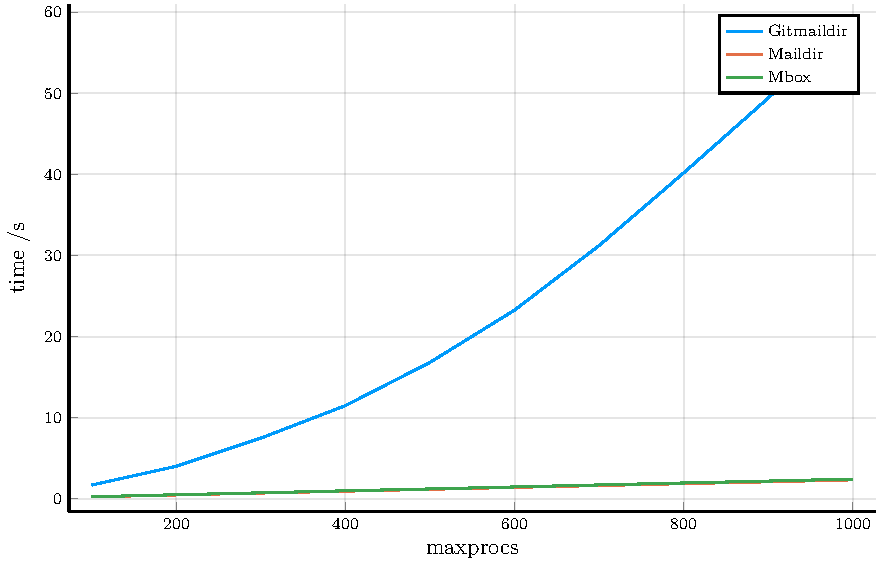
\includegraphics{figs/tds_combined}
    \input{figs/tds_combined.pdf_tex}
    \caption{The time taken to deliver 1000 emails sequentially for Gitmaildir, Maildir, and Mbox. Ribbon represents 95\% confidence interval (it is very narrow and so hard to see).}
    \label{fig:tds_combined}
\end{figure}


\begin{figure}[h]
    \centering
    %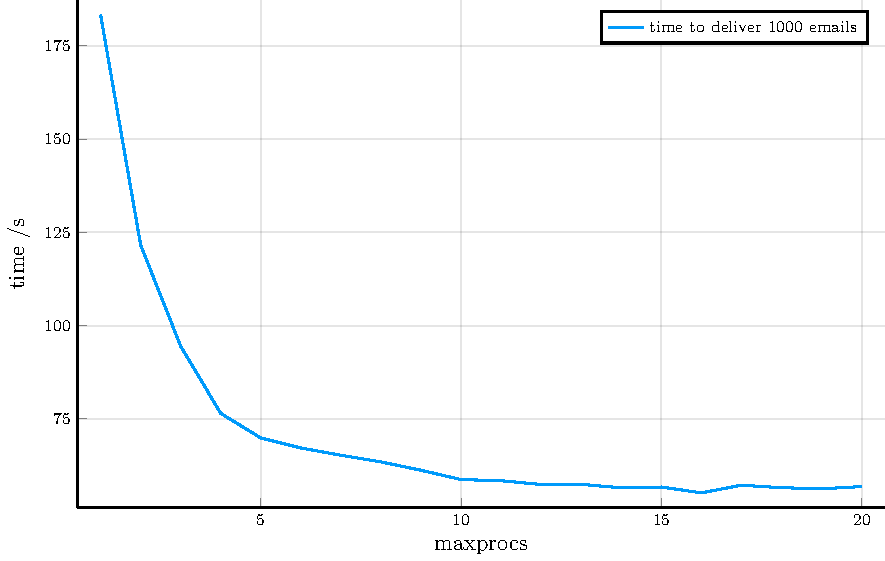
\includegraphics{figs/tdpp}
    \input{figs/tdpp.pdf_tex}
    \caption{The time taken to deliver 1000 emails at different levels of parallelism for Gitmaildir. Ribbon represents 95\% confidence interval.}
    \label{fig:tdpp}
\end{figure}

For a program that is completely parallel we would expect a straight line, so when the plot starts to veer from this line and eventually become flat we can see where the sequential code becomes a bottleneck. The speedup graph for Gitmaildir can be seen in figure \ref{fig:tdpp_speedup}. From this graph we can see that Gitmaildir starts to slow at around 5 threads. I think that this was due to the locking when making commits as that is the only part of the code that is required to be sequential and so it is probably the bottleneck under highly parallel loads.

\begin{figure}[h]
    \centering
    %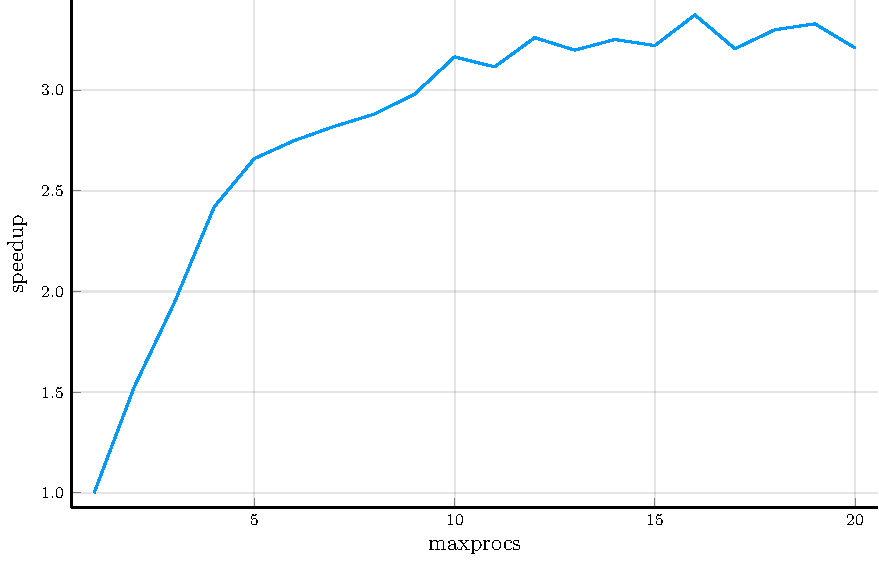
\includegraphics{figs/tdpp_speedup}
    \input{figs/tdpp_speedup.pdf_tex}
    \caption{The speedup in time taken to deliver 1000 emails at different levels of parallelism for Gitmaildir. Ribbon represents 95\% confidence interval.}
    \label{fig:tdpp_speedup}
\end{figure}

A similar graph for standard Maildir and Mbox can be seen in figure \ref{fig:tdpp_speedup_combined}. As expected, the line produced for Maildir is straight. This is because for delivery Maildir has no sequential operations at all meaning that processes can run in parallel as long as there are enough cores. On the other hand, the result for Mbox is surprising, being also a straight line even though accesses to the mailbox must be sequential. I hypothesise that this was because although the accesses themselves must be sequential, appending to a file is a very fast operation, especially when the volume of data is not too great. Therefore most of the time is spent preparing to write to the file, for example when reading in the data and opening the file, meaning that even though the access itself is purely sequential, the act of delivering data has other parts which are parallelisable and are the majority of the workload in the instance of delivering an email. Overall from this graph, we can see that when it comes to speedup, Gitmaildir vastly underperforms when compared to Maildir and Mbox.

\begin{figure}[h]
    \centering
    %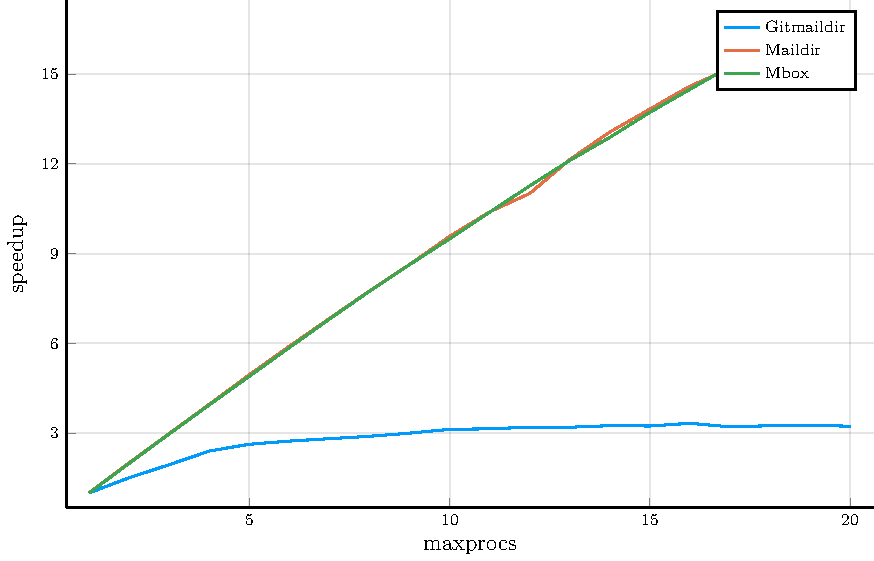
\includegraphics{figs/tdpp_speedup_combined}
    \input{figs/tdpp_speedup_combined.pdf_tex}
    \caption{The speedup in time taken to deliver 1000 emails at different levels of parallelism for Gitmaildir, Maildir and Mbox. Ribbon represents 95\% confidence interval.}
    \label{fig:tdpp_speedup_combined}
\end{figure}

It is also important to compare the raw speeds as well as speedup, and we can see that Gitmaildir also underperforms here. We can see in figure \ref{fig:tdpp_combined} that Gitmaildir is much slower (around ten times) than Mbox and Maildir even when running in parallel. This is unsurprising given that it is doing far more work. For each deliver, Gitmaildir writes to three files, performs three hashes and also has to encode the data and this does not include reading from the store at the start. Mbox and Maildir both only need to write raw data into a single file. However the real problem seems to be that it does not benefit from being more parallel even as much as Mbox does.

\begin{figure}[h]
    \centering
    %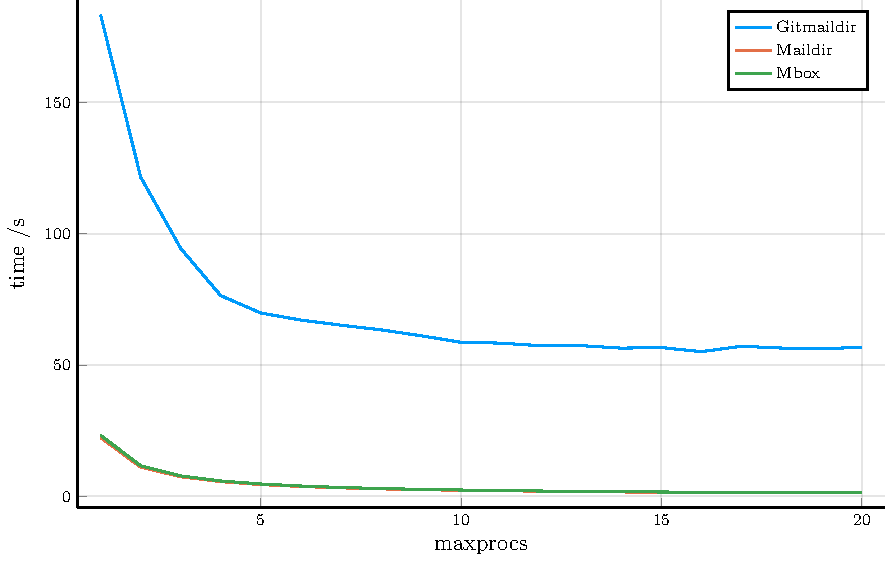
\includegraphics{figs/tdpp_combined}
    \input{figs/tdpp_combined.pdf_tex}
    \caption{The time taken the deliver 1000 emails at different levels of parallelism for Gitmaildir, Maildir and Mbox. Ribbon represents 95\% confidence interval.}
    \label{fig:tdpp_combined}
\end{figure}

\begin{figure}[h]
    \centering
    %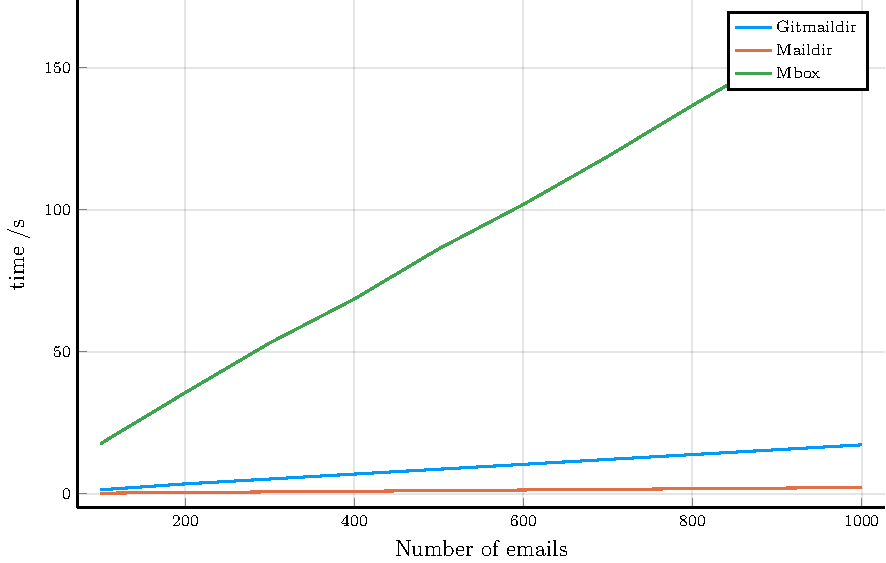
\includegraphics{figs/tmp_combined}
    \input{figs/tmp_combined.pdf_tex}
  \caption{The time taken to change the metadata of different numbers of emails for Gitmaildir, Maildir and Mbox. Ribbon represents 95\% confidence interval (it is very narrow and so hard to see).}
    \label{fig:tmp_combined}
\end{figure}

As well as email delivery, I looked into the performance of editing email metadata. This differs from delivery because it involves retrieving the correct email in the mailbox and modifying it in someway (a write into the file for Mbox, a filename change for the other two). Figure \ref{fig:tmp_combined} shows how the different mailboxes performed at a fixed level of parallelism. We can see a very different result here to before. Whereas for deliver Gitmaildir was significantly slower than the other two, it is now Mbox that is significantly slower (roughly 5 times slower than Gitmaildir and 10 times slower than Maildir). This comes down to the fundamental difference between how the two systems store email and email metadata. For Maildirs, because its flags are on the end of the filename we do not have to open files and then search inside them unlike Mbox. The greatest speedup probably can be attributed then to the fact that an Mbox is not indexed, and although a Maildir is not explicitly indexed either\footnote{Some implementations, notably Dovecot\cite{dovecot_maildir}, actually do lock the Maildir to provide an index, however this means that we immediately lose its concurrency benefit.}, the directory itself is what makes it much faster to get to the email to modify.

\begin{figure}[h]
    \centering
    %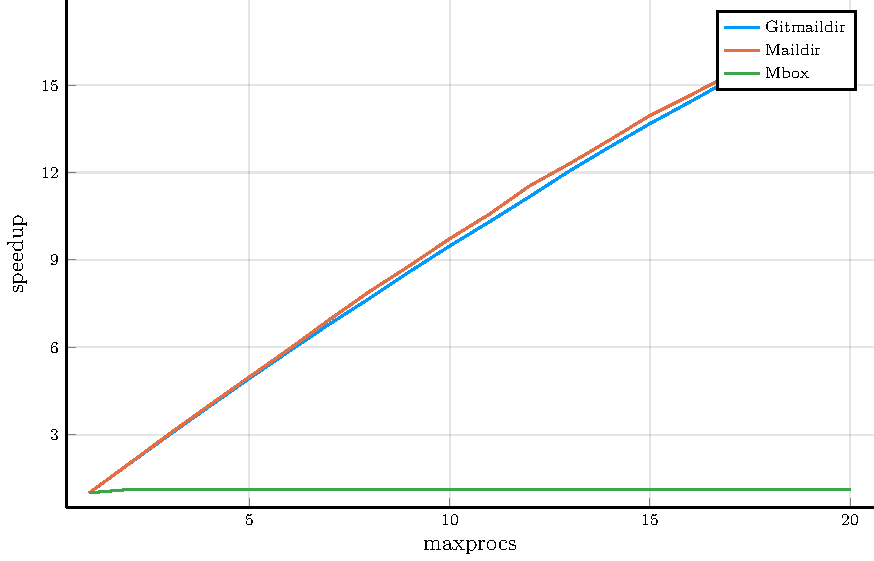
\includegraphics{figs/tmpp_speedup_combined}
    \input{figs/tmpp_speedup_combined.pdf_tex}
    \caption{The speedup in time taken to change the metadata of 1000 emails at different levels of parallelism. Ribbon represents 95\% confidence interval.}
    \label{fig:tmpp_speedup_combined}
\end{figure}

As before I also measured how the different mailboxes performed at different levels of parallelism. We can see in figure \ref{fig:tmpp_speedup_combined} that the lines for both Gitmaildir and Maildir are almost straight matching the equation $y=x$ which shows that they are both able to fully exploit the parallelism. On the other hand the line for Mbox is flat which means that for this metric it is not able to exploit any parallelism at all because the majority of the time is spent reading and writing the mailbox which is sequential. This matches the expected findings and shows that Gitmaildir in this case has managed to inherit the benefits provided by the Maildir specification while still maintaining strong consistency. When compared to the delivery test, I think that this shows Gitmaildir maintains its parallel advantage as long as the operation being performed on the mailbox is sufficiently long-running.

\subsection{Test conditions and caveats}

For all of the above tests I tried to make sure that the testing conditions were fair across the different mailbox types and would be useful for real usage. There are of course a few caveats to the methods that I will mention. First, the filesystem format used will have made a difference to the results because filesystems perform different types of indexing and storage. My choice of tmpfs was made specifically to remove disk access latency from being included in my timing, but as most mailboxes are stored in normal disk space such as ext4 the indexing may cause timing differences unrelated to disk accesses. There is also the question of whether testing parallelisation using xargs provides accurate results. It will add overhead that I may have been able to avoid through a different method, however it will be the same overhead for all the tests so the comparisons should still be fair.

\subsection{Summary of results}

From the performance testing and comparisons with Maildir and Mbox, I have been able to show that, as expected, Maildir is faster for most operations than my Gitmaildir implementation. Also, Mbox is significantly faster in some places but not in others. This is the cost of extra features which may outweigh some of the performance disadvantages. However, whether this is actually a problem depends on how these tests map into real world usage. Most mailboxes do not receive thousands of emails all at once, so the time it takes to perform actions on a Gitmaildir are probably acceptable for more standard use (this would of course need verifying with data on it being used in a real-world application). Another point to take into account is that the parallelisation tests were performed with one to twenty cores. Most personal machines at the moment currently have around 2-8 cores and so any speedup after that point is not so useful outside of the server environment.

\section{Success criteria}

\subsection{Successful functionality}

The first success criterion stated that the project would be evaluated against:

\begin{quote}
  Implementation of a working Git overlay on top of the filesystem in MirageOS.
\end{quote}

This was provided by the operations that I built on top of the ocaml-git library allowing a mixture of Git plumbing commands and Git porcelain commands to be executed in OCaml. The unit tests prove that the functionality works. As ocaml-git works on MirageOS (it was written as part of the MirageOS project) then a library that uses it as the backend will also work on MirageOS so the second part of the criterion is satisfied. This has been checked on MirageOS by writing a simple application that commits a file to a Git store using my library and it worked successfully. As the rest of ocaml-git works on MirageOS and my library passes all the unit tests, it can be inferred that my Git overlay will work on top of the filesystem in MirageOS.

Therefore, the first of the two success criteria has been met.

\subsection{Strong consistency}

The second success criterion stated that the project would be evaluated against:

\begin{quote}
  A strongly consistent Maildir index using the Git overlay which allows all standard Maildir operations.
\end{quote}

I will start by addressing the first half of this criterion. It requires that the application provides a strongly consistent overlay on top of Maildir. As described before, the application records each operation as a separate Git commit in a single local Git repository. Strongly consistent can be defined as:
\begin{quote}
  All accesses are seen by all parallel processes (or nodes, processors, etc.) in the same order (sequentially).
\end{quote}
Because each operation is stored in a separate commit and we have a single main branch, that means that we have a single ordering of all operations which is seen by all users of the Gitmaildir. This means that we have a total ordering of all actions and so they are seen by all parallel processes in the same order, matching our definition above.

The second half of this criterion specifies the application must allow all standard Maildir operations. I have taken this to mean the ones I defined in my requirements analysis. So I have also met this part of the criterion. However, as the Gitmaildir is a standard Maildir structure in a Git repository, any other features that do not require non-standard extensions can be easily added by manipulating the Maildir like a Git standard Git repository.

Therefore, the second of the success criteria has been met and so both of the success criteria have been met meaning that my project has successfully achieved its original aims.

\section{Extensions}

The first extension was to implement a plugin system for Gitmaildir. I succeeded in this which can be seen by the fact that the second extension was possible which was to build a plugin for Gitmaildir. The plugin system has the benefit that it was written in such a way to be easily extensible itself. It would be fairly straightforward to add different ways of loading and configuring plugins at runtime for example.

The second extension was to build a plugin that creates a mirror mailbox where each email is converted to plain text. This was built, and upon testing with a repository of real emails they were successfully converted to plain text in a separate branch (which is how the plugin maintains the mirror repository). However, it is possible that there are edge cases I do not account for which will lead to some parts of the email not being converted to plain text.
